\documentclass[../Lael_John_MasterThesis_Draft.tex]{subfiles}
\graphicspath{\subfix[../images]}
\begin{document}
%   FORMALLY DEFINE/HIGHLIGHT ORDER DEFINITION
\section{Tensors in an Algebraic Setting}\label{section:tensoralgebra}
The most abstract way of thinking about tensors is when describing them as elements of a tensor product of modules. Consider $A, B$ and $P$ as being modules over a ring $R$. Then any bi-linear mapping, $t: A \times B \to P$, is described by acting on elements from $A \times B$ in the following  manner: 
\begin{equation*}
    t(\lambda a, b) = t(a, \lambda b) = \lambda t(a, b), a \in A, b \in B, \lambda \in R, t(a,b) \in P
\end{equation*}

\begin{figure}[h]
    % https://q.uiver.app/#q=WzAsMyxbMCwwLCJBIFxcdGltZXMgQiJdLFsyLDAsIlAiXSxbMSwxLCJBIFxcb3RpbWVzX1IgQiJdLFswLDEsImZcXDsgXFx0ZXh0e211bHRpbGluZWFyfSA9IFxcdGlsZGV7Zn0gXFxjaXJjIFxcdmFycGhpIl0sWzAsMiwiXFx2YXJwaGkiLDJdLFsyLDEsIlxcZXhpc3RzICFcXHRpbGRle2Z9IiwyXV0=
    \[\begin{tikzcd}
        {A \times B} && P \\
        & {A \otimes_R B}
        \arrow["{t\; \text{bilinear} = \tilde{t} \circ \varphi}", from=1-1, to=1-3]
        \arrow["\varphi"', from=1-1, to=2-2]
        \arrow["{\exists !\tilde{t}}"', from=2-2, to=1-3]
    \end{tikzcd}\]
    \caption{Illustrating a tensor product of $R$-modules}\label{fig:tensorcommutativediagram}
\end{figure}

Such a bilinear, or even generalising to a multi-linear, mapping between $R$-modules can be represented by an element lying in their tensor product, such that \Cref{fig:tensorcommutativediagram} commutes \cite{vakil_rising_2025} (illustrated specifically for the case mentioned above). Such a tensor product of $R$-modules is unique up to unique isomorphisms, and this is referred to in algebraic literature as a \textit{universal property} of tensor products.  

% This act of representing any such bilinear mapping via an element of the tensor product is commonly referred to as a \textit{universal property} in algebra.

While such an abstract description is useful when showing that any general elements lying in the specified spaces $A$ and $B$ can be combined to form a tensor, it does not specify details required for showing how this tensor can be represented. 

A more useful approach to understanding tensors is to begin from a foundation in linear algebra. As matrices represent linear transformations between vector spaces $V$ and $W$, so $d$-way arrays can be used to represent multilinear relationships between vector spaces $V_1, V_2 \ldots V_d$, where each $V_i$ has a dimension $n_i$. Diving deeper into this analogy, a matrix of the form $n_i \times n_j$ behaves either as a  bilinear map from the product $V_i^* \times V_j \to \mathbb{F}$, or as linear map $V_j \to V_i$ or as its dual $V_i^* \to V_j^*$. This hybrid nature of matrices is a reflection of the underlying fact that matrices represent order-$2$ tensors. Since computing elements $A_{ij}$ of the matrix $A$ depends on a choice of bases for both vector spaces $V$ and $W$, an analogous choice of bases must be made when representing a $d$-linear tensor, $T \in V_1 \otimes V_2 \otimes \cdots \otimes V_d$, as a $d$-way array.

\nomenclature[B]{$V_i$}{A vector space over $\field$ having dimension $n_i$}%
\nomenclature[B]{$V_i^*$}{The dual vector space to $V_i$}%
For the purposes of this thesis, unless specified, each vector space will be considered over a field $\field = \reals$ or $\complex$. Here each vector space $V_i$ is equipped with its standard basis, $\{e_{i,j}\}_{j=1}^{n_i}$, where $e_{i,j}(k) = \delta_{j,k}$. Each different choice of basis changes how the tensor $T$ is represented as a $d$-way array.

\nomenclature[C]{$e_{i,j}$}{The $j$-th standard ordered basis vector in $V_i$. The $i$ may not be dropped if it is clear from context}
\nomenclature[C]{$v(k)$}{The $k$th entry in a vector $v$}
\begin{definition}[Order of a Tensor]\label{defn:tensororder}
    An element lying in the tensor product of $d$ vector spaces, $T \in V_1 \otimes \cdots\otimes V_d$, is said to be an \textbf{order-$d$ tensor}.
\end{definition}
Consider $T := v_1 \otimes \cdots \otimes v_d$, a specific order-$d$ tensor, with each component vector $v_i \in V_i$. Then, in coordinates $$v_i = \sum_{j=1}^{n_i} v_i(j)e_{i,j}, \; v_i(j) \in \field \;\forall j = 1, \ldots, n_i.$$
%  with components $v_i(j)$ according to the standard ordered basis of the corresponding vector space.
  The elements of a $d$-way array that corresponds to $T$ then can be given in the following manner: $$T(k_1, k_2, \ldots, k_d) = \prod_{i=1}^{d} v_i(k_i),$$where $1 \leq k_i \leq n_i$. 
%   --- the dimension of each corresponding vector space $V_i$.

\nomenclature[D]{$T(k_1,\ldots, k_d)$}{The element located at the position $(k_1, \ldots, k_d)$ in a tensor $T$}

In a similar fashion, given two tensors in $V_1 \otimes \cdots \otimes V_d$ of the specific form $T_1:= v_1 \otimes \cdots \otimes v_d$ and $T_2:= w_1 \otimes \cdots \otimes w_d$, then one can describe the $d$-way array corresponding to the tensor $T_1 + T_2$ in coordinates as follows $$(T_1 + T_2)(k_1, k_2, \ldots, k_d) = \left(\prod_{i=1}^{d} v_i(k_i)\right) + \left(\prod_{i=1}^{d} w_i(k_i)\right),$$indicating simply a componentwise addition in the corresponding $d$-way arrays. A similar description can be made when scaling a tensor by any factor $\lambda \in\field$ --- $\lambda T$.

Therefore an order $d$ tensor $T \in V_1 \otimes \cdots \otimes V_d$ that can be expressed as a sum of these specific \textit{elementary} forms, as above, can also be represented by a $d$-way array. This property is satisfied by any general order-$d$ tensor (see \Cref{defn:decomposition}).
\begin{definition}[Modes of a Tensor]
    % For a tensor $T \in V_1 \otimes \cdots \otimes V_d$, the \textbf{modes} of $T$ refer to the $d$ distinct vector spaces $V_i, i = 1, \ldots, d$ required to construct $V_1 \otimes \cdots \otimes V_d$
    Given an order-$d$ tensor, $T \in V_1 \otimes \cdots \otimes V_d$, the modes of $T$ refer to specifying the $d$ distinct ways that $T$ as a tensor can be oriented. Thus a tensor of order $d$ has exactly $d$ modes.
    %  indices that make up the tuples indicating elements in the $d$-way array that represents $T$. [IS THERE A WAY TO MAKE THIS DEFINITION INDEPENDENT OF COORDINATES?]
\end{definition}
\begin{remark}
    % When specific mode of a tensor $T \in V_1 \otimes \cdots \otimes V_d$ is mentioned, this can be visualised as specifying an orientation for $T$. If $T$ can be represented as a $d$-way array, then the $i$-th mode corresponds to treating the $i$-th element in the indexing tuple as fixed.
    Modes of are useful because they provide a specific orientation along which operations can be performed on a given tensor. When working with tensors as $d$-way arrays, the  modes can be seen as the distinct indices in the overall tuples that index the elements of the array.
\end{remark}
\begin{example}
    Consider $$T:= (a,b,c,d)\otimes(x,y,z)\otimes(p,q) \in \field^4 \otimes \field^3 \otimes \field^2.$$Then $T$ is an order-$3$ tensor having $3$ modes. Each entry in the $3$-way array representing $T$ is indexed by a tuple $(i_1,i_2,i_3) \in [4] \times [3] \times [2].$
\end{example}
\nomenclature[A]{$[n]$}{The set $\{1, 2, \ldots, n\}$, (see \Cref{defn:tensorformat})}
\begin{definition}[Format of a Tensor]\label{defn:tensorformat}
    For a given tensor $T \in V_1 \otimes \cdots \otimes V_d$, the format of $T$ refers to the tuple $(n_1, \ldots, n_d)$, conveying all the possible indices of the $d$-way array that represents $T$. For any two tensors lying in the same tensor space, their formats are the same. Here, the $n_i$ are exactly the dimensions of $V_i$.
\end{definition}
% \vspace{12pt}
% \hrule
\subsection*{Viewing Tensors}
A tensor $T:= v_1 \otimes \cdots \otimes v_d \in V_1 \otimes \cdots \otimes V_d$ can be viewed in the following different ways \cite{landsberg_tensors_2012}: \begin{enumerate}\label{list:viewingtensors}
    \item As a multilinear mapping between $V_1^* \times V_2^* \times \cdots \times V_d^* \to \mathbb{F}$ (extending the analogy of looking at matrices as order-$2$ tensors) $$(f_1, f_2 \ldots f_d) \mapsto \prod_{i=1}^{d} f_i(v_i).$$ Here $f_i \in V_i^*$, the dual space to each vector space $V_i$.
    \item For every choice of $i\in \{1, \ldots, d\}$, $T$ can be viewed as a linear mapping from $V_i^* \to V_{\hat{i}} := V_1 \otimes \cdots \otimes V_{i-1} \otimes V_{i+1} \otimes \cdots \otimes V_d$. Viewing $T$ this way takes a vector (an order-$1$ tensor) to an order-$(d-1)$ tensor. \begin{equation}\label{eqn:tensormappingdroporder}
        f_j \mapsto f_j(v_i)(v_1 \otimes \cdots \otimes v_{i-1}\otimes v_{i+1} \otimes \cdots \otimes v_d).
    \end{equation}
    This viewpoint can be seen when defining an operation that selects a specific "slice" of a tensor (or even a linear combination of them), after fixing the mode $i$.
    % This viewpoint can be seen in \Cref{subsection:tensorslicing}, slicing the tensor along the $i$th mode, and in \Cref{subsection:tensorflattening} as the columns of the flattening operation.
    \nomenclature[B]{$V_{\hat{i}}$}{The tensor product of vector spaces excluding $V_i$, defined as $V_1 \otimes \cdots \otimes V_{i-1} \otimes V_{i+1} \otimes \cdots \otimes V_d$}
    \item Finally, as the dual of the defined linear map (see \Cref{eqn:tensormappingdroporder}), now going from $V_{\hat{i}}^* \to V_i$. This point of view of transforms an order-$(d-1)$ tensor to a rescaling of the vector $v_i$. $$f_1 \otimes \cdots \otimes f_{i-1} \otimes f_{i+1} \otimes \cdots \otimes f_d \mapsto \left(\prod_{j \neq i} f_j(v_j)\right)v_i.$$Here note that the dual operation and the tensor product operation commute.
\end{enumerate}

Each of these different viewpoints holds for order-$d$ tensors in general, not just for these specific elementary tensors. This becomes evident in the following section on tensor rank and decompositions.
% Each of these above viewpoints also corresponds to an appropriate output to the transformation of the representative $d$-way array chosen: either to a scalar, a $(d-1)$-way array or a vector respectively \cite{landsberg_tensors_2012}. In fact scalars and vectors can be defined as tensors of orders $0$ and $1$ respectively.

% \vspace{12pt}
% \hrule
% \section{Tensors in a Geometric Setting}\label{section:tensorgeometry}
% The existence of such a mapping allows for non-zero order-$d$ tensors (of the same form as \cref{defn:elementarytensors}) to be represented as points lying on this new \textit{Segre variety}.

% \begin{lemma}
%     The Segre mapping as defined above is an injective map, but not surjective.
% \end{lemma}
% \begin{proof}
%     This mapping is well defined (all tuples have an image in $\proj V$, and the image of a tuple is unique). However, the Segre mapping is generally not surjective. Not every point in $\proj V$ can be written as the image of a single tuple of the form $([v_1], \ldots, [v_d])$. A simple example is when dealing with $3 \times 3$ matrices $[e_1 \otimes e_1 + e_2 \otimes e_2]$ cannot be written as the image of a single tuple of $([v_1], [v_2])$. 

%     Starting with two distinct tuples $([a_1], \ldots, [a_d])$ and $([b_1], \ldots, [b_d])$ gives us at least one pair of vectors $a_i, b_i$ that do not lie on the same line through the origin in $V_i$. The resulting images under $\Sigma$ are the tensors $[a_1 \otimes \cdots \otimes a_d]$ and $[b_1 \otimes \cdots \otimes b_d]$ that differ at least in one component in the $d$-way arrays, and therefore represent distinct families of tensors. Thus the Segre mapping is injective, and ends up being referred to as the Segre \textit{embedding} in algebraic geometry litereature.
% \end{proof}

% %DOES IT MAKE SENSE TO DISCUSS THE GEOMETRIC IMAGES OF THE FLATTENINGS/SLICES?
% \subsection*{Why is it important to consider both?}
% Both aspects prove useful as tools to study tensors. Explicit computation is far easier when working with tensors algebraically, and thus much more easily applicable in fields other than mathematics, once problems have been stated in appropriate terms. On the other hand, dealing with the geometry of tensors allows for a much better examination of edge cases and boundary conditions, particularly useful when working with proofs about general properties that should apply to tensors. 

\section{Rank}\label{section:tensorrank}
The first key focus of Comon's conjecture involves figuring out how tensors can be built. The following example shows that there exist tensors that cannot be written as simply the tensor product of vectors analogously to how not all vectors in a vector space can be written as rescaled basis vectors.
\begin{example}
    When dealing with $2 \times 2$ matrices $\in \field^2 \otimes \field^2$, consider $e_1 \otimes e_1 + e_2 \otimes e_2$ (the identity matrix). Such a matrix cannot be written as $v_1 \otimes v_2$, a simple tensor product of two vectors, where $v_1, v_2 \in \field^2$. 
\end{example}
Making this preliminary observation leads to the following definition ---
\begin{definition}[Elementary Tensor]\label{defn:elementarytensors}
    Consider an order-$d$ tensor, $T$, of the specific form $T:= v_1 \otimes \cdots \otimes v_d \in V_1 \otimes \cdots \otimes V_d$. Since $T$ can be written explicitly as the tensor product of $d$ vectors, it is called an \textbf{elementary tensor}. Equivalent names for such tensors in the literature reviewed are \textit{rank-$1$} tensors and \textit{decomposable} tensors.
\end{definition}
% The Segre Variety (as defined in \cref{defn:segremapping}) contains exactly the images of all the non-zero \textit{elementary} tensors in a given tensor product. This still leaves open the question of how tensors of higher rank can be represented, which has been tackled successfully in the literature by the developement of \textit{secant varieties} \cite{bernardi_hitchhiker_2018} (see \cref{section:pastoverview})

Using these elementary tensors as building blocks provides a way to describe the construction of any general order-$d$ tensors. In the most naive way, this can be done by considering all elementary tensors of the form $e_{1, j_1} \otimes \cdots \otimes e_{d, j_d}$. This explains why any general order-$d$ tensor can be represented by a $d$-way array, and also why the three viewpoints specified above for an elementary tensor can be extended to a general order-$d$ tensor.
\begin{definition}[Tensor Decomposition \cite{zhang_comons_2016}]\label{defn:decomposition}
    Consider any order-$d$ tensor $T \in V_1 \otimes \cdots \otimes V_d$. A \textbf{decomposition} of $T$ consists of writing $T$ as a sum of elementary tensors $$T = \sum_{k=1}^{s} \lambda_k v_1^k \otimes \cdots \otimes v_d^k,$$ with each of the $v_i^k \in V_i$ and $\lambda_k \in \field$.
\end{definition}
\nomenclature[C]{$v_i^k$}{The $k$-th vector lying in $V_i$}
\begin{remark}
    Here note that there exist multiple names for describing the decomposition of a tensor into the sum of elementary tensors - polyadic forms, canonical decomposition (CANDECOMP), parallel factors (PARAFAC) etc. The above definition agrees with what is known in the literature as CP-decomposition (a combination of names CANDECOMP/PARAFAC). \cite{kolda_tensor_2009}
\end{remark}
Thus, for any given tensor $T$, there can exist multiple decompositions, not just depending on the choice of basis vectors for each $V_i$. Two questions naturally follow this definition of tensor decomposition: \begin{description}
    \item[Q1.] For a given order-$d$ tensor $T$, does there exist a shortest decomposition?
    \item[Q2. ] If such a shortest decomposition exists, is it unique (up to the choice of a different set of basis vectors)?
\end{description}
The answer to the first question can be given in terms of the following definition:
\begin{definition}[Tensor Rank]\label{defn:tensorrank}
    The \textbf{rank} of a tensor $T$, denoted $\rank(T)$, is the minimal length of any possible decomposition of $T$.
\end{definition}
\nomenclature[F]{$\rank(T)$}{The rank of a tensor $T$}
\nomenclature[F]{$\srank(T)$}{The symmetric rank of a symmetric tensor $T$}
A rank decomposition of a tensor always exists, because tensors can always be written in terms of elementary tensors. Computing the rank of a given tensor is not an easy problem, but there exist multiple approaches in the literature that rely on both the algebraic properties of tensors and associated transformations, and the geometric properties of the varieties on which these tensors lie. Tensor rank also does not depend on which elementary tensors are involved in a decomposition. Thus Q1 as given above has an affirmative answer, but Q2 does not --- multiple rank decompositions can exist for a specified tensor.

% A further question that can be asked is regarding the limiting behaviour of a sequence of tensors, leading to the following definition. 
% \begin{definition}[Border Rank]\label{defn:borderrank}
%     A tensor $T$ has border rank $r$ if it can be expressed as a limit of a sequence of tensors of rank $r$, but not for any sequence of tensors with rank $s < r$. Conventional notation is to denote border rank with $\underbar{\rank}(T) = r$
% \end{definition}
% The notion of border rank comes in use when working with secant varieties, as a tool to help compute rank. Tensors can have differing ranks and border ranks
% \begin{example}[\cite{landsberg_tensors_2012}] 
%     Consider $T:= a_1 \otimes b_1 \otimes c_1 + a_1 \otimes b_1 \otimes c_2 + a_1 \otimes b_2 \otimes c_1 + a_2 \otimes b_1 \otimes c_2$ Then the rank of this tensor is 3, but one can write $T$ as the limit of tensors of rank 2 in the following manner $$T(s) = \frac{1}{s}\left((s-1)a_1 \otimes b_1 \otimes c_1 + (a_1 + sa_2)\otimes (b_1 + sb_2) \otimes (c_1 + sc_2)\right)$$ 
% \end{example} 


\section{Symmetric Tensors}\label{section:symmetrictensors}
The other focus of Comon's Conjecture revolves around tensors that exhibit the property of symmetry. These tensors become valuable in applications simply because the symmetry means that they require "less" information to be constructed. What makes a tensor symmetric is the next logical question to tackle, and it becomes necessary to define how permutations act on a given tensor.

Given $\sigma \in S_d$ (the symmetry group of $\{1, 2, \ldots , d\}$), the permutation action of $\sigma$ on a tensor $T$ can be defined as follows:
\begin{definition}[Permutation of a Tensor]\label{defn:tensorpermutation}
    % Let $T \in \underbrace{V \otimes \cdots \otimes V}_{\text{$d$ times}}$. Then $\sigma \in S_d$ acts on $T$ (represented as a $d$-way array) in the following manner $$\sigma \cdot T(k_1, k_2, \ldots k_d) = T(\sigma(k_1), \sigma(k_2), \ldots, \sigma(k_d))$$ 
    % [THE ABOVE DEFINITION IS IN COORDINATES. REWRITING THIS IN GENERAL]
    Let $T \in V_1 \otimes \cdots \otimes V_d$ be an order-$d$ tensor. Then $\sigma \in S_d$ acts on all tensors in $V$ by linearly extending the following mapping of elementary tensors:
    $$\sigma: V_1 \otimes \cdots \otimes V_d \to V_{\sigma_1} \otimes \cdots \otimes V_{\sigma_d}, v_1 \otimes \cdots \otimes v_d \to v_{\sigma_1} \otimes \cdots \otimes v_{\sigma_d}.$$ This induces a corresponding mapping from a general $T \mapsto \sigma \cdot T := \sigma \cdot \left( \sum_{i=1}^{r} T_i\right)$, where each $T_i$ is an elementary tensor.
\end{definition}
\nomenclature[A]{$\sigma$}{A permutation of a finite collection of elements (the length of the collection is specified in context)}
% Note here that all the vector spaces are the same, to keep this permutation mapping well defined. 
To talk about tensors being invariant under permutation actions, it is necessary to work with tensors that retain the same format after permutation. This means symmetric tensors can only exist in the space $V^{\otimes d}:= \underbrace{V \otimes \cdots \otimes V}_{\text{$d$ times}}$. These tensors are sometimes referred to in the literature as being \textit{cubical}.
% If the vector spaces were allowed to differ in dimension, then this would no longer be a group action, since the underlying set keeps changing (shuffling around.)
% This fact also allows for the use of notation $T \in V^{\otimes d}$. 
% Such tensors are also referred to as \textit{cubical}.

The definition of a symmetric tensor now follows: 
\begin{definition}[Symmetric Tensor \cite{comon_symmetric_2008}]\label{defn:symmetrictensor}
    Consider a tensor $T \in V^{\otimes d}$. $T$ is said to be \textbf{symmetric} if the following is true: \begin{equation}\label{eqn:symmetrictensordefn}
        T = \sigma \cdot T \; \forall \; \sigma \in S_d.
    \end{equation}
\end{definition}
\begin{remark}
    As a consequence of this definition, the following equivalent equality condition also holds for symmetric tensors $$T = \frac{1}{d!} \sum_{\sigma \in S_d} \sigma \cdot T.$$ This gives rise to an operator that transforms any tensor into a symmetric tensor. 
\end{remark}
\begin{definition}[Symmetrisation Operator]\label{defn:symmetrisationoperator}
    Let $T \in V:= V_1 \otimes \cdots \otimes V_d$ be an order-$d$ tensor. Then the \textbf{symmetrisation operator} is defined as follows:
    \begin{equation}\label{eqn:symmetrisationoperatordefn}
        \mathcal{S}: V \to V,\; T \mapsto \frac{1}{d!} \sum_{\sigma \in S_d} \sigma \cdot T.   
    \end{equation} 
    The resulting tensor $\mathcal{S}(T)$ is always symmetric.
\end{definition}
\nomenclature[E]{$\mathcal{S}(T)$}{The symmetrisation operator (see \Cref{defn:symmetrisationoperator}) acting on a tensor $T$}%
Since every tensor can be expressed as a sum of elementary tensors (see \Cref{defn:decomposition}), $\rank(T)$ is defined for symmetric tensors $T$ as well. However, one can define \textit{elementary symmetric tensors} as tensors in $V^{\otimes d}$ of the form $v^{\otimes d}$ where $v \in V$. Establishing this definition allows for symmetric tensors to be written as a sum of these elementary symmetric tensors, resulting in the definition of \textbf{symmetric decompositions} and the analogous notion of \textbf{symmetric rank}, denoted $\srank(T)$. The following lemma (Lemma 4.2 in \cite{comon_symmetric_2008}) shows why such a symmetric decomposition always exists for a symmetric tensor $T$.
\begin{lemma}[\cite{comon_symmetric_2008}]\label{lemma:symmetricdecompositionexistence}
    Let $T$ be a symmetric, order-$d$ tensor lying in $(\field^n)^{\otimes d}$. Then there exist vectors $v_1, \ldots, v_s \in \field^n$, and $\lambda_1, \ldots, \lambda_s \in \field$ such that 
    \begin{equation}\label{eqn:symmetrictensordecomposition}
        T = \sum_{i=1}^{s} \lambda_iv_i^{\otimes d}.
    \end{equation}
\end{lemma}
% \begin{proof}
%     Suppose the lemma is false. Then there must exist a symmetric, order-$d$ tensor $T$ that cannot be expressed in the form $\sum_{i=1}^{s} v_i^{\otimes d}$ for any $s > 0$. Then $T$ can only be expressed as an infinite sum of symmetric tensors. Now each term in this infinite expansion is of the form $\lambda_iv_i^{\otimes d}$. $(\field^n)^{\otimes d}$ is a finite dimensional vector space. Since the space $V_1 \otimes \cdots \otimes V_d$ is finite dimensional, such a sum can be expressed in a finite manner, leading to a contradiction of the initial assumption that the lemma was false.
%     Therefore, a symmetric decomposition must always exist for $T$, a symmetric order-$d$ tensor.
% \end{proof}
\begin{remark}
    The proof given in \cite{comon_symmetric_2008} involves showing that the space generated by all $k$-th tensor powers of linear forms in the symmetric tensors cannot be contained in any non-zero non-trivial hyperplane. Their proof also involves defining a bilinear form on the space of the symmetric tensors (see \Cref{defn:bilinearformhompoly}).
\end{remark}
\begin{example}
    Consider the tensor\begin{eqnarray*}
        T &:=& (1,0,0) \otimes (1,0,0) \otimes (1,0,0) + (0,0, 1) \otimes (0,0,1) \otimes (0,0,1)\\ && + (0,1,0) \otimes (0,1,0) \otimes (0,1,0)\\
        &=& (1,0,0)^{\otimes 3} + (0,0, 1)^{\otimes 3} + (0,1,0)^{\otimes 3}.
    \end{eqnarray*} This is definitely a symmetric decomposition, and $T$ is a symmetric tensor.
\end{example}
It is clear that not every tensor can be seen as symmetric, and therefore the subset of all order-$d$ tensors that are symmetric is denoted $S^d(\field^n) \subsetneq (\field^n)^{\otimes d}$ --- notation usually reserved for homogeneous polynomials in $n$ variables of fixed degree $d$. In fact it can be shown that these spaces, $S^d(\field^n)$ and $\field[x_1, \ldots, x_n]_d$, are isomorphic to each other. This isomorphism is a powerful tool that allows for an interchange of polynomial and tensor notation (in an appropriate manner) when dealing with symmetric tensors.
\nomenclature[B]{$S^d(\field^n)$}{Symmetric tensors (forms) of order $d$ over $\field^n$}

% \vspace{12pt}
% \hrule
\subsection*{Symmetric Tensors and Homogenous Polynomials of Fixed Degree}\label{subsection:homogeneouspolyrelation}
A homogeneous polynomial $f \in \field[x_1, \ldots, x_n]_d$ is of the form \begin{equation}\label{eqn:hompolynomialexpandeddefn}
    f(x_1, \ldots x_n) = \sum_{a_i \geq 0, \sum_{i}^{n} a_i = d} \lambda_{(a_1, \ldots, a_n)}\prod_{i=1}^{n}x_i^{a_i},
\end{equation}
where all the coefficients $\lambda_{(a_1, \ldots, a_n)} \in \field$. The following notation is also standard in the literature surveyed, taking $\mathbf{x} := (x_1, x_2, \ldots x_n)$ to be the tuple of variables and the tuple of exponents denoted $\mathbf{\alpha}:= (a_1, a_2, \ldots a_n) \in (\naturals \cup \{0\})^n$. Then one has $\mathbf{x^{\alpha}} := \prod_{i=1}^{n}x_i^{a_i}$. Further $|\mathbf{\alpha}| = \sum_{i}^{n} a_i$, so the homogeneous polynomial in \Cref{eqn:hompolynomialexpandeddefn} can be rewritten as 
\begin{equation}\label{eqn:hompolynomialconddefn}
    f(\mathbf{x}) = \sum_{|\mathbf{\alpha}| = d} \lambda_{\mathbf{\alpha}}\mathbf{x^{\alpha}}.
\end{equation}
\nomenclature[A]{$\field[x_1, \ldots, x_n]_d$}{Subring of polynomial ring in $n$ variables over $\field$, consisting of polynomials of fixed degree $d$}
\nomenclature[C]{$\mathbf{x}$}{A vector of indeterminates $(x_1, \ldots, x_n)$}
\nomenclature[C]{$\mathbf{\alpha}$}{A vector of non-negative integers $(a_1, \ldots, a_n)$}
\nomenclature[C]{$\mathbf{x^{\alpha}}$}{$\prod_{i=1}^{n} x_i^{a_i}$ where $n$ is taken from context}
\nomenclature[C]{$|\alpha|$}{The sum of all elements in $\mathbf{\alpha}$}
The following proposition is standard in tensor decomposition literature, but is stated again for convenience.
\begin{proposition}\label{prop:homotensorisomorphism}
    For fixed values of $d, n > 0$, the map $$\Phi_d: \field[x_1, \ldots, x_n]_d \to S^d(\field^n),$$ defined by linearly extending the following mapping of the degree-$d$ monomials
    \begin{equation}\label{eqn:hompolytosymtensormapping}
        \mathbf{x^{\alpha}} \mapsto \frac{1}{d!}\sum_{\sigma \in S_d} \sigma \cdot \left(\bigotimes_{i=1}^n e_i^{\otimes a_i}\right) = \mathcal{S}\left(\bigotimes_{i=1}^n e_i^{\otimes a_i}\right),
    \end{equation}
    is an isomorphism of vector spaces over $\field$.
\end{proposition}
\begin{proof}
    Each degree-$d$ monomial, $\mathbf{x}^{\alpha}$, can be seen as a basis vector in the vector space $\field[x_1, \ldots, x_n]_d \cong \field^{\binom{n+d-1}{d}}$. These monomials are mapped to symmetric tensors, by the definition of the symmetrisation operator (see \Cref{defn:symmetrisationoperator}). $\Phi_d$ is thus a well-defined mapping, since all other homogeneous degree-$d$ polynomials can be constructed as linear combinations of these basis vectors. Therefore for $\lambda \in \field$,
    
    $$\Phi(\lambda \mathbf{x^{\alpha}} + \mathbf{x^{\beta}}) = \lambda \left( \frac{1}{d!}\sum_{\sigma \in S_d} \sigma \cdot (\bigotimes_{i=1}^n e_i^{\otimes a_i})\right) + \left( \frac{1}{d!}\sum_{\sigma \in S_d} \sigma \cdot (\bigotimes_{i=1}^n e_i^{\otimes b_i})\right) = \lambda\Phi(\mathbf{x^{\alpha}}) + \Phi(\mathbf{x^{\beta}}). $$

    Further, every elementary symmetric tensor $v^{\otimes d} = (\sum_{i=1}^{n}v_ie_i)^{\otimes d}$ can be seen as the image of the $d$-th power of the linear form $\left(\sum_{i=1}^{n} v_ix_i \right)^d$. Since every symmetric tensor has a symmetric tensor decomposition, $\Phi_d$ must also be surjective. 
    

    % Finally, consider two homogeneous polynomials $f(\mathbf{x}) := \sum_{|\alpha| = d} f_{\alpha} \mathbf{x}^{\alpha}$ and $g(\mathbf{x}):= \sum_{|\alpha| = d} g_{\alpha} \mathbf{x}^{\alpha}$ such that $f_{\alpha}, g_{\alpha} \in \field\;\forall\;\alpha$, and $\Phi_d(f(\mathbf{x})) = \Phi_d(g(\mathbf{x}))$. This is equivalent to saying \begin{eqnarray*}
    %     &&\Phi_d(\sum_{|\alpha| = d} f_{\alpha} \mathbf{x}^{\alpha}) = \Phi_d(\sum_{|\alpha| = d} g_{\alpha} \mathbf{x}^{\alpha})\\
    %     &\iff& \sum_{|\alpha| = d} f_{\alpha} \Phi_d(\mathbf{x}^{\alpha}) = \sum_{|\alpha| = d} g_{\alpha} \Phi_d(\mathbf{x}^{\alpha})\\
    %     &\iff& \sum_{|\alpha| = d}  \frac{f_{\alpha}}{d!}\sum_{\sigma \in S_d} \sigma \cdot \left(\bigotimes_{i=1}^n e_i^{\otimes a_i}\right) = \sum_{|\alpha| = d}  \frac{g_{\alpha}}{d!}\sum_{\sigma \in S_d} \sigma \cdot \left(\bigotimes_{i=1}^n e_i^{\otimes a_i}\right)\\
    %     &\iff& \sum_{|\alpha| = d}  \frac{(f_{\alpha} - g_{\alpha})}{d!}\sum_{\sigma \in S_d} \sigma \cdot \left(\bigotimes_{i=1}^n e_i^{\otimes a_i}\right) = 0\\
    %     &\iff& f_{\alpha} = g_{\alpha} \;\forall\; |\alpha| = d
    % \end{eqnarray*}
    % and this is enough to say that $f(\mathbf{x}) = g(\mathbf{x})$, showing that $\Phi$ is an injective function.Thus there exists an isomorphism between these two vector spaces.
    % Finally consider $f \in \field[x_1, \ldots x_n]_d$ lying in the kernel of $\Phi_d$. This implies $\Phi_d(f) = 0$, a symmetric order-$d$ tensor. Thus we have 
    % Suppose $\Phi_d$ is not injective. Then there exist $f, g \in \field[x_1,\ldots,x_n]_d$ such that $\Phi_d(f) = \Phi_d(g)$ but $f \neq g$. Now if $f \neq g$, then there is at least one coefficient $\alpha^{\prime}$ such that $f_{\alpha'} \neq g_{\alpha'}$. Without a loss of generality, let this be the only index where the functions are not equal. Now we definitely have that $\Phi_d(f)-\Phi_d(g) = 0$, by our assumption. This is equivalent to the following $$\sum_{|\alpha| = d}\frac{f_{\alpha} - g_{\alpha}}{d!}\sum_{\sigma \in S_d} \sigma \cdot \left(\bigotimes_{i=1}^n e_i^{\otimes a_i}\right) = 0.$$ But this simplifies to the following expression $$\frac{f_{\alpha'} - g_{\alpha'}}{d!}\left(\sum_{\sigma \in S_d} \sigma \cdot \left(\bigotimes_{i=1}^n e_i^{\otimes a_i}\right)\right) = 0,$$a contradiction, because none of the tensors on the left side of the multiplication are 0, and by the initial assumption, the fraction must also be non-zero, and this multiplication is occurring in an integral domain. Thus the initial assumption must be false, and $\Phi_d$ must be injective.

    It remains to show that $\Phi_d$ is injective. Consider two monomials $\mathbf{x}^{\alpha}$ and $\mathbf{x}^{\beta}$, where $\alpha \neq \beta$ i.e. they differ at at least one index. Then the tensors they map to, $\Phi_d(\mathbf{x}^{\alpha}) := \mathcal{S}\left(\bigotimes_{i=1}^n e_i^{\otimes a_i}\right)$ and $\Phi_d(\mathbf{x}^{\beta}) := \mathcal{S}\left(\bigotimes_{i=1}^n e_i^{\otimes b_i}\right)$ are symmetric, but they are not linear multiples of each other, since they are composed of distinct elementary symmetric tensors. In fact, for any collection of distinct indices $\lambda \in \naturals \cup \{0\}$, the monomials $\mathbf{\lambda}$ must all map to symmetric tensors that are linearly independent. Since the monomials are now seen to be linearly independent, consider an element $f \in \field[x_1, \ldots, x_n]_d$ to lie in the kernel of $\Phi_d$. This means that $\Phi_d(f) = 0$. But $f$ can be written as $f = \sum_{|\alpha| = d} f_{\alpha}\mathbf{x}^{\alpha}$, where all the ${\alpha}$ are distinct. 

    Then since $\Phi_d(f) = 0$, this is the same as writing $$\sum_{|\alpha| = d} f_{\alpha}\Phi_d(\mathbf{x}^{\alpha}) = 0.$$
    Since the images of all the monomials under $\Phi_d$ are linearly independent (they are all monomials indexed by distinct $\alpha$), the only way this equation holds is if all the coefficients $f_{\alpha} = 0$. Thus $f$ being in the kernel of $\Phi_d$ necessitates it being the $0$ polynomial, showing that $\Phi_d$ is injective. 
\end{proof}
In fact $\Phi_d$ can be seen as a component of a larger isomorphism between graded vector spaces, $\Phi: \oplus_{i \geq 0}\field[x_1, \ldots, x_n]_i \to \bigoplus_{d \geq 0} S^d(\field^n)$ \cite{comon_symmetric_2008}. 

% \subsection*{Symmetric Tensors and the Veronese Mapping}\label{subsection:veronesemapping}
% In addition to being in bijection with homogeneous polynomials of fixed degree, as a result of their symmetry, symmetric tensors can be seen as points in a space of much lower dimension. As earlier, this allows for the elementary symmetric tensors to be mapped to a variety. 
% Since non-zero elementary symmetric tensors are of the form $\left(\sum_{i=1}^{n}v_ie_i\right)^{\otimes d}$ this mapping embeds the constituent vectors into the Veronese variety. \cite{oeding_report_2008} As previously, this mapping is not surjective.

% Since $\binom{n+d-1}{d} < (n)^d$ for all $d > 1, n > 1$, we know that the Veronese variety lies in a lower dimensional space than the Segre, and a mapping can be constructed to see the image of $\nu_d(\proj\field^n) \in \Sigma(\proj \field^n \times \cdots \times \proj\field^n)$ since elementary symmetric tensors are also tensors. In fact the image of the diagonal $\Delta := \{([x], \ldots, [x])| [x] \in \proj \field^n \}$ under the Segre mapping is exactly the embedding of the Veronese into the Segre mapping. 

% Armed with this background of symmetric tensors and rank, and with an understanding of how to view tensors as both multi-way arrays, some of them as homogeneous polynomials, and some of them as points in space, the next step to be taken in this thesis is to cover the literature around Comon's Conjecture.

\section{The Geometry of Tensors}\label{section:tensorgeometry}
Tensors are not just algebraic objects, but also points lying in a space equipped with a topology and geometry. Just as vectors and matrices can be seen as points lying in a vector space, higher-order tensors can be viewed in a similar manner. 

Since general tensors can be built out of elementary ones, it makes sense to first see how these can be visualised. By the multi-linear nature of tensors, any elementary tensor $T$ of the form $v_1 \otimes \cdots \otimes v_d \in V_1 \otimes \cdots \otimes V_d$ is non-zero if and only if all of the component vectors $v_i$ are non-zero. It is also convenient to work with the elementary tensors up to scalar multiplication, leading to the use of the projective space $\proj V$, denoting the set of all lines passing through the origin of the vector space $V$. Such a space is usually seen to be equipped with the Zariski topology.

The map from $V_i \setminus \{0\} \to \proj V_i$ is defined as taking $v_i \mapsto [v_i(1): \ldots :v_i(n)]$ where the image is expressed in homogeneous coordinates. Note here that when moving to the $\proj V_i$, even though the number of coordinates used to describe $v_i$ is $n_i$, the space $\proj V_i$ has dimension $(n_i - 1)$.

The component vectors of $T$ can now be written as a tuple lying in the Cartesian product of $d$ projective spaces i.e. $([v_1], \ldots, [v_d]) \in \proj V_1 \times \cdots \times \proj V_d$. Writing this tuple as a point in a higher dimensional projective space is exactly the goal of defining the Segre mapping (also known as the Segre \textit{embedding}).
\begin{definition}[Segre Mapping \cite{smith_invitation_2004}]\label{defn:segremapping}
    Define $\Sigma: \proj V_1 \times \cdots \times \proj V_d \to \proj V$ as the following mapping $$([v_1], \ldots, [v_d]) \mapsto [v_1 \otimes \cdots \otimes v_d].$$The image point lies in the projectivisation of $V$, a vector space over $\field$ of dimension $\prod_{i=1}^{d} n_i$. The complete image $\Sigma(\proj V_1 \times \cdots \times \proj V_d) \subsetneq \proj V$ is called the \textit{Segre variety}. 
\end{definition}
\begin{remark}
    All points on the Segre variety correspond to the non-zero elementary tensors in $V_1 \otimes \cdots \otimes V_d$, up to scalar multiplication. 
\end{remark}
Visualising a general order-$d$ tensor with respect to the points on the Segre embedding first requires the definition of a secant variety. Such a construction arises by extending the idea of constructing secant lines to a curve, or secant planes to a surface to higher dimensions. 
\begin{definition}[$r$-th Secant Variety \cite{bernardi_hitchhiker_2018}]\label{defn:rsecantvariety}
    Let $X \subset \proj V$ be a projective variety. Then the $r$-th secant variety to $X$, denoted $\sigma_r(X)$ is defined as
    \begin{equation}\label{eqn:rsecantvariety}
        \sigma_r(X) := \overline{\bigcup_{x_1, \ldots, x_r \in X} \langle x_1, \ldots, x_r \rangle}.
    \end{equation}
    Here $\langle x_1, \ldots, x_r \rangle$ denotes the smallest projective linear space containing the points $\{x_i\}_{i=1}^r$. The bar denotes the Zariski closure in $\proj V$, covering the cases where the points $x_i$ chosen may lie on the same $k$-hyperplane, where $k < r$. In particular this construction includes all possible tangent $k$-hyperplanes to $X$.
\end{definition}
\begin{remark}
    Note here that for $r < s$, it is evident that $\sigma_r(X) \subseteq \sigma_s(X)$.
\end{remark}
% Using this definition, a rank-$r$ tensor of order-$d$, $T$, should lie in the projective linear span of $\{x_1, \ldots, x_r\} \subset \Sigma(\proj V_1 \times \cdots \times \proj V_d)$,and thus must lie in $\sigma_r(\Sigma(\proj V_1 \times \cdots \times \proj V_d))$.  

Consider $T$ to be a tensor of order $d$ and rank $r$. Then $T$ can be expressed as a linear combination of $r$ elementary tensors, and therefore must lie in their linear span. Thus $T$ can be visualised as lying in $\sigma_r(\Sigma(\proj V_1 \times \cdots \times \proj V_d))$, and not in any $\sigma_s(\Sigma(\proj V_1 \times \cdots \times \proj V_d))$, when $s < r$. This lowest $r$ can also be written as $\rank_{\Sigma(\proj V_1 \times \cdots \times \proj V_d)}([T])$, where $[T]$ denotes the projective image of the tensor $T$.
\begin{remark}
    The space $\sigma_r(\Sigma(\proj V_1 \times \cdots \times \proj V_d))$ also contains more tensors than just those having rank $r$, since the definition of secant varieties involves taking the closure of a set. However, the collection of points lying in $\sigma_r(\Sigma(\proj V_1 \times \cdots \times \proj V_d))$, representing tensors of rank $r$ forms a dense subset. Thus it is seen as convenient in the literature to use secant varieties to model problems about decompositions \cites{ballico_tensor_2013, bernardi_hitchhiker_2018}.
\end{remark}
\begin{figure}
    \centering
    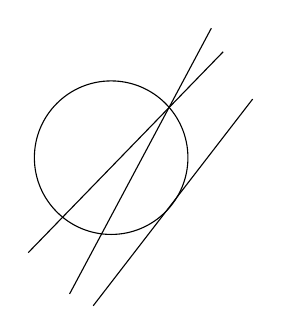
\begin{tikzpicture}[scale=0.3]
        % Coordinates
        \coordinate (A) at (4.51, 6.52);
        \coordinate (B) at (4.51, 6.52);
        \coordinate (C) at (1.00, 2.50);
        \coordinate (D) at (9.25, 11.00);
        \coordinate (E) at (2.75, 0.75);
        \coordinate (F) at (8.75, 12.00);
        \coordinate (G) at (3.75, 0.25);
        \coordinate (H) at (10.50, 9.00);

        % Drawing
        \draw (A) circle (3.25);
        \draw (C) -- (D);
        \draw (E) -- (F);
        \draw (G) -- (H);
    \end{tikzpicture}
    \caption{Secant lines through a circle (and a limiting tangent line)}\label{figure:secantexample}
\end{figure}
At the start of \Cref{section:symmetrictensors}, the idea that symmetric tensors require less information in their construction was floated, and this can be seen with the help of the Veronese mapping (also known as the Veronese \textit{embedding}).
\begin{definition}[Veronese Mapping]\label{defn:veronesemapping}
    Define the mapping $\nu_d:\proj \field^n \to \proj \field^{\binom{n + d - 1}{d}}$ in the following manner $$[v(1): \ldots : v(n)] \mapsto [v(1)^d: v(1)^{d-1}v(2): \ldots : v(n-1)v(n)^{d-1}:v(n)^d], $$where $v \in \field$ and $v(i)$ are the components of the vector. The complete image $\nu_d(\proj\field^n) \subset \proj\field^{\binom{n+d-1}{n}}$ is known as the \textit{Veronese variety.}
\end{definition}
\begin{remark}
    It is a well-established fact in algebraic geometry that the $d$-th Veronese variety $\nu_d(\proj V)$ can be seen as lying inside the Segre variety of $d$ copies of $\proj V$, $\Sigma(\proj V \times \cdots \times \proj V)$. This is in line with the algebraic notion of $S^d(V) \subset V^{\otimes d}$.
\end{remark}
\begin{remark}
    As with tensors of rank $r$ being visualised as lying in $\sigma_r(\Sigma(\proj V_1 \times \cdots \times \proj V_d))$, a similar operation can be applied to show that symmetric tensors of symmetric rank $r$ lie in $\sigma_r(\nu_d(\proj V))$.
\end{remark}

\section{Working with Tensors}
The questions of how tensors are constructed and where they live have been addressed in the preceding sections. The goal of this final section of the chapter is to provide the necessary tools and terminology required when performing tensor analysis.
\subsection{Slicing a Tensor}\label{subsection:tensorslicing}
When working with lower-order tensors like matrices, columns or rows can be viewed as linearly dependent or independent, and this has an effect on the rank of the matrix. This behaviour is ideal an an analogy to describe higher-order tensors as composed of lower-order slices. Conventionally the columns of a matrix would be the $1$-slices, since they occur along the "first" mode, and the rows would therefore be considered $2$-slices.
\begin{definition}[Slices of a Tensor]\label{defn:tensorslicing}
    % Let $T:= v_1 \otimes \cdots \otimes v_d \in V_1 \otimes \cdots \otimes V_d$ be an elementary, order-$d$ tensor. Here each $v_i \in V_i$, with $V_i$ a vector space with dimension $n_i$. 
    
    % Then, \textbf{the $j$-th $i$-slice of $T$} is given by
    % $$T_j^i:= (v_i)(j)(v_1 \otimes \cdots v_{i-1} \otimes v_{i+1} \cdots \otimes v_d)\in V_{\hat{i}}.$$
    % Here $1 \leq j \leq n_i$. For each \textit{mode} $1 \leq i \leq d$, there are $n_i$ order-$(d-1)$ slices that make up $T$. \\
    % This definition is equivalent to selecting the $j$-th $i$-slice of the $d$-way array that represents $T$. For a general tensor $T \in V_1 \otimes \cdots \otimes V_d$, the slice $T^i_j$ is exactly the sum of the $j$-th $i$-slices of elementary tensors that make up a rank decomposition of $T$.
    % \hrule
    Let $T \in V_1 \otimes \cdots \otimes V_d$ be a general order-$d$ tensor. Then $T$ admits a rank decomposition $$T := \sum_{i=1}^{r} v_1^i \otimes \cdots \otimes v_d^i, \; v_j^i \in V_j \;\forall\; j = 1, \ldots, d.$$Then the \textbf{$j$-th slice along the $k$-th mode} (also called the $j$-th $k$-slice) is an order-$(d-1)$ tensor, lying in $V_{\hat{k}}$, given by the following formula: $$T_j^k := \sum_{i=1}^{r}v_k(j) (v_1^i \otimes \cdots \otimes v_{k-1}^i \otimes v_{k+1}^i \otimes \cdots \otimes v_d^i).$$In this definition, $1 \leq j \leq n_k$ since these slices are indexed up to the dimension of $V_k$.
    
    When viewing $T$ as a multi-way array, the $j$-th $k$-slice is equivalent to working with the $(d-1)$-way array, generated by fixing the $k$-th index in the original $d$-way array. $$T_j^k(\lambda_1, \ldots, \lambda_{k-1},\lambda_{k+1},\lambda_d) = T(\lambda_1, \ldots, \lambda_{k-1}, j, \lambda_{k+1}, \ldots, \lambda_d)$$
\end{definition}
\nomenclature[D]{$T^i_j$}{The $j$-th slice along the $i$-th mode of a tensor $T$ (see \Cref{defn:tensorslicing})}
\begin{observation}
    This definition of the $j$-th $k$-slice cannot be made coordinate-independent. The various $k$-slices are differentiated by the fact that as a vector $v_k^i = (v_k^i(j))_{j=1}^{n_k}$, and this representation depends on a choice of basis for $V_k$. Since $V_k \cong \field^{n_k}$, unless another basis is specified, the standard basis $\{e_j\}_{j=1}^{n_k}$ is used.
\end{observation}
\begin{remark}
    Through the rest of this thesis, the superscript accompanying a tensor variable, written in uppercase roman letters, indicates the chosen mode along which a specified operation must occur.
\end{remark}
\begin{example}
    \begin{figure}[h]
        \centering
        \begin{tikzpicture}[scale=0.85]
            \definecolor{darkgreen}{RGB}{0,113,0}
    
            % Coordinates
            \coordinate (A) at (1.00, 8.00);
            \coordinate (B) at (1.97, 9.00);
            \coordinate (C) at (4.00, 8.00);
            \coordinate (D) at (4.98, 9.02);
            \coordinate (E) at (4.00, 4.00);
            \coordinate (F) at (5.00, 5.00);
            \coordinate (G) at (1.50, 8.50);
            \coordinate (H) at (4.50, 8.50);
            \coordinate (I) at (4.50, 4.50);
            \coordinate (J) at (2.00, 8.00);
            \coordinate (K) at (2.00, 4.00);
            \coordinate (L) at (3.00, 8.00);
            \coordinate (M) at (3.00, 4.00);
            \coordinate (N) at (3.00, 9.00);
            \coordinate (O) at (4.00, 9.00);
            \coordinate (P) at (1.00, 7.00);
            \coordinate (Q) at (4.00, 7.00);
            \coordinate (R) at (5.00, 8.00);
            \coordinate (S) at (1.00, 6.00);
            \coordinate (T) at (4.00, 6.00);
            \coordinate (U) at (5.00, 7.00);
            \coordinate (V) at (1.00, 5.00);
            \coordinate (W) at (4.00, 5.00);
            \coordinate (X) at (5.00, 6.00);
            \coordinate (Y) at (1.71, 9.51);
            \coordinate (Z) at (6.00, 7.00);
            \coordinate (AA) at (9.00, 10.00);
            \coordinate (AB) at (7.25, 7.00);
            \coordinate (AC) at (7.75, 10.00);
            \coordinate (AD) at (12.97, 7.04);
            \coordinate (AE) at (7.50, 7.00);
            \coordinate (AF) at (7.50, 7.00);
            \coordinate (AG) at (9.00, 4.00);
            \coordinate (AH) at (8.25, 7.00);
            \coordinate (AI) at (7.25, 4.00);
            \coordinate (AJ) at (13, 10.47);
            \coordinate (AK) at (18, 6.80);
            \coordinate (AL) at (14.5, 3.55);
    
            % Drawing
            \draw (1,4) rectangle (4,8);
            \draw (A) -- (B);
            \draw (C) -- (D);
            \draw (E) -- (F);
            \draw[darkgreen, very thick] (B) -- (D);
            \draw[darkgreen, very thick] (F) -- (D);
            \draw[darkgreen, very thick, dashed] (G) -- (H);
            \draw[darkgreen, very thick, dashed] (H) -- (I);
            \draw[blue, very thick, dashed] (J) -- (K);
            \draw[blue, very thick, dashed] (L) -- (M);
            \draw[blue, very thick, dashed] (J) -- (N);
            \draw[blue, very thick, dashed] (L) -- (O);
            \draw[dashed] (P) -- (Q);
            \draw[dashed] (Q) -- (R);
            \draw[red, very thick, dashed] (S) -- (T);
            \draw[red, very thick, dashed] (T) -- (U);
            \draw[red, very thick, dashed] (V) -- (W);
            \draw[red, very thick, dashed] (W) -- (X);
            \node[above] at (Y) {$T \in \mathbb{F}^4 \otimes \mathbb{F}^3 \otimes \mathbb{F}^2$};
            \draw (Z) .. controls (7.25, 7.00) and (7.75, 10.00) .. (AA);
            \draw (Z) .. controls (7.50, 7.00) and (7.50, 7.00) .. (AD);
            \draw[red] (9.5,9) rectangle (11.5,12);
            \draw (13,9) rectangle (13,9);
            \draw[blue] (14,5) rectangle (16,9);
            \draw[darkgreen] (9.5,2) rectangle (12.5,6);
            \draw (Z) .. controls (8.25, 7.00) and (7.25, 4.00) .. (AG);
            \node[above] at (AJ) {$T^1_3 \in \mathbb{F}^3 \otimes \mathbb{F}^2$};
            \node[above] at (AK) {$T^2_2 \in \mathbb{F}^4\otimes \mathbb{F}^2$};
            \node[above] at (AL) {$T^3_2 \in \mathbb{F}^4\otimes \mathbb{F}^3$};
        \end{tikzpicture}
        \caption{Slicing a tensor $T \in \field^4\otimes\field^3\otimes\field^2$ along different modes}\label{figure:slicingtensor}
    \end{figure}
    Consider a tensor $T \in \field^4\otimes\field^3\otimes\field^2$, where $T := (1,2,3,4) \otimes (1,2,3) \otimes (1,2)$. Then slices along different modes are computed as follows (visualised in \Cref{figure:slicingtensor}) \begin{itemize}
        \item $T^1_3 = 3((1,2,3) \otimes (1,2))$
        \item $T_2^2 = 2((1,2,3,4) \otimes (1,2))$
        \item $T^3_2 = 2((1,2,3,4) \otimes (1,2,3))$
    \end{itemize}
\end{example}
% \begin{observation}
%     Slicing in the above definition is described for only an elementary order $d$ tensor, but it is a linear operation (addition and scalar multiplication don't change it.)
% \end{observation}
% \begin{observation}
%     The operation defined above for taking the $j$-th $i$-slice of an order-$d$ tensor,  $S^i_j: V:= V_1 \otimes \cdots \otimes V_d \to V_{\hat{i}}$ defined as $T \mapsto T^i_j$ is a well-defined linear mapping between vector spaces, by \Cref{defn:tensorslicing}.
% \end{observation}
\begin{definition}[Slicing Operator]\label{defn:slicingoperator}
    Given the space $V_1 \otimes \cdots \otimes V_d$, and integers $1 \leq k \leq d$ and $1 \leq j \leq n_k$, define the operation $$S_j^k:V_1\otimes \cdots \otimes V_d \to V_{\hat{k}}, T\mapsto T_j^k.$$Such an operator is well-defined, and is, in fact, a linear operator. 
\end{definition}
\nomenclature[E]{$S^i_j(T)$}{The mapping that selects the $j$-th slice along the $i$-th mode of a tensor $T$ (see \Cref{defn:slicingoperator})}
% \begin{proof}
%     Let $T:= \otimes_{i=1}^d v_i \in V$ be an elementary tensor. Then $S^i_j(T)$ exists and lies in the appropriate $V_{\hat{i}}$. Further for $T_1 = T_2 \in V$ one has $S^i_j(T_1) = S^i_j(T_2)$ by applying the definition provided above. Consider $S^i_j(T_1 + T_2)$. Then the $j$-th $i$-slices of the d-way array $T_1 + T_2$ are exactly given by $f_j(v_i)(v_{\hat{i}}) + f_j(w_i)(w_{\hat{i}})$ where $v_i, w_i \in \field^{n_i}$ and $v_{\hat{i}}, w_{\hat{i}} \in V_{\hat{i}}$. Thus $S^i_j$ as an operation preserves addition. Likewise $S^i_j(\lambda T) = \lambda(S^i_j(T)) = \lambda T^i_j$, preserving scalar multiplication. Therefore $S^i_j$ is a linear operation $V \to V_{\hat{i}}$.
% \end{proof}

% \begin{lemma}\label{lemma:rankrelationshipwithonemode}
%     Given a tensor $T \in V_1 \otimes \cdots\otimes V_d$, such that $\rank(T) = r \leq \max_{1 \leq i \leq d} n_i$, then there is at least one mode $1 \leq i \leq d$ having $r$ linearly independent slices $T^i_j$ where $1 \leq j \leq n_i$.
% \end{lemma}
% \begin{proof}
%     Suppose the claim is false i.e. there is no mode $i$ such that the number of linearly independent slices $T^i_j$ is $r$. Since we are only dealing with a finite order $d$, there is a mode $i$ with the largest number of linearly independent slices $T^i_j$. Let this number be $\rho$. By the initial supposition, one must have:
%     \begin{description}
%         \item[$\rho < r$:] Each of the slices $S^j_i(T) = T_j^i$ can be written as a linear combination of exactly $\rho$ slices of order $(d-1)$. One can therefore rewrite the decomposition of $T$ in terms of vectors in $V_i$ and the linearly independent set of $S^i_j(T)$, a decomposition of length less than $r$, contradicting the definition of $r = \rank(T)$. 
%         \item[$\rho > r$:] Then any decomposition of $T$ with length $r$ must miss out at least one of the linearly independent slices that make up $T$, a contradiction to the initial idea of decomposing $T$.
%     \end{description}
%     Thus the assumption of the claim being false leads to a contradiction in either case. Therefore $\rho = r$, for at least one mode $i$.
% \end{proof}

% \begin{corollary}
    % Given a tensor $T$ of rank $r$, the collections of slices $\{T^i_j\}_{j=1}^{n_i}$ along all modes $1 \leq i \leq d$ have $r$ linearly independent elements, i.e $\langle T^i_j \rangle_{j=1}^{n_i}$ is an $r$-dimensional subspace.
% \end{corollary}
\nomenclature[B]{$\langle v_i \rangle_{i=1}^n$}{The linear span of $n$ vectors}
A major claim from the literature on Comon's conjecture is the following theorem about the number of linearly independent slices along a chosen mode, when working with rank decompositions. The theorem as stated below first appeared as Lemma 3.1 in \cite{zhang_comons_2016}, but in a more geometric formulation it was proved earlier as Proposition 2.4 in \cite{buczynski_ranks_2013}. The proof given below seeks a balance between these two formulations.
\begin{theorem}[\cite{zhang_comons_2016}, \cite{buczynski_ranks_2013}]\label{thm:ranklinearindependentslices}
    Let $T$ be an order-$d$ tensor of rank $r$. Then a rank decomposition of $T$ is given as $$T := \sum_{k=1}^{r} v_1^k \otimes \cdots \otimes v_d^k.$$ For any mode $i$, the set of slices $$\{ v_1^k \otimes \cdots\otimes v_{i-1}^k \otimes v_{i+1}^k \otimes \cdots \otimes v_d^k \in V_{\hat{i}} \;|\; 1 \leq k \leq r \}$$ is linearly independent.
\end{theorem}
\begin{proof}
    Let $1 \leq i \leq d$ be fixed, as an arbitrary mode for this proof. Then the tensor $T \in V_i \otimes V_{\hat{i}}$. Define a curve 
    \begin{equation}
        S(t):= \sum_{k=1}^{r} v^k_i(t) \otimes v_{\hat{i}}^k(t),\; S(0) = T.
    \end{equation}
    Here $v_i^k(t)$ are curves in $V_i$, and $v_{\hat{i}}^k(t)$ are curves in $V_{\hat{k}}$. One can restrict to working with $V_i^{\prime} \subset V_i$ instead of $V_i$, while keeping $S(t) \in V_i^{\prime} \otimes V_{\hat{i}}$. This can also be followed by assuming that $S(t): V_i^* \to V_{\hat{i}}$ an injective mapping, when $t$ is sufficiently close to $0$. Then since $T(V_i^*)$ can be written as $\lim_{t \to 0} S(t)(V_i^*) \subseteq \lim_{t\to 0} \langle v_{\hat{i}}^k(t) \rangle_{k=1}^r$, one has $\rank(T(V_i^*)) \leq \rank(T)$.
    
    Conversely, consider a set $w_{\hat{i}}^k(t) \subset V_{\hat{i}}$ such that $T(V_i^*) \subset \lim_{t\to 0} \langle w_{\hat{i}}^k \rangle_{k=1}^r$, where the dimension of the span of $w_{\hat{i}}^k(t)$ is assumed to be constant. Then, considering a basis $\{f_{i,j}\}_{j=1}^{n_i}$ of $V_i^*$ (dual to the basis $\{e_{i,j}\}_{j=1}^{n_i} \subset V_i$), one can write $$T(f_{i,j}) = \lim_{t \to 0} \sum_{k=1}^{r} \lambda_{j,k}w_{\hat{i}}^k(t),$$ for functions $\lambda_{j,k}(t)$. Then the tensor $T$ can be written as $$T = \sum_{j=1}^{n_i} e^j_i \otimes \left[\lim_{t\to 0}\sum_{k=1}^{r}\lambda_{j,k}(t)w_{\hat{i}}^k(t)\right].$$ Here the $\lambda_{j,k}(t)$ are appropriately chosen functions. By the multilinear nature of tensor products, this can be rewritten as $$S(t) = \sum_{k=1}^{r} \left[\sum_{j=1}^{n_i}\lambda_{j,k}e_i^j(t)\right] \otimes w_{\hat{i}}^k(t).$$At $t \to 0$, this forms a decomposition of $T$ which must necessarily be at least as long as the rank decomposition of $T$. Thus $\rank(T) \leq \rank(T(V_i^*))$. 

    Since $\rank(T) = \rank(T(V_i)^*)$, consider the mapping from $V_i^* \to V_{\hat{i}}$, given by $f \mapsto T(f)$. Here $T(f) = (\sum_{k=1}^r v_1^k \otimes \cdots \otimes v_d^k)(f)$, which simplifies to $T(f) = \sum_{k=1}^{r} f(v_i^k)v_{\hat{i}}^k$. If the set $B = \{v_{\hat{i}^k}\}_{k=1}^r \subset V_{\hat{i}}$ forms a basis for $T(V_i^*)$, then the proof is complete. It is clear that $B$ spans all of $T(V_i^*)$, by the definition of the linear map $T: V_i^* \to V_{\hat{i}}$.
    But the $\rank(T(V_i^*))$ is equal to $\dim T(V_i^*)$, the dimension of the linear subspace generated in $V_{\hat{i}}$. A spanning set lying in $T(V_i^*)$ with $\dim T(V_i^*) = r$ elements forms a basis for $T(V_i^*)$, and must therefore be linearly independent. Therefore $B$ as a set is linearly independent.  
\end{proof}
% What other major theorems/lemmas do we need to establish about slicing tensors?
% What are the properties of slicing?
% What does slicing look like in geometry?

\begin{remark}
    When working with $T \in V_1 \otimes \cdots \otimes V_d$, a general tensor, then the format of $S_j^k(T)$ - the $j$-th $k$-slice of $T$ is a tuple of length $d-1$, contained in the format of $T$.
\end{remark}
% \begin{remark}
%     When working with symmetric tensors $T \in S^d(V) \subset V^{\otimes d}$ the operation of taking slices $S_j^{k_1}(T) = S_j^{k_2}(T)$ for all $1 \leq k_1 \leq k_2 \leq d$ and a fixed $0 < j \leq \dim V$. This is by the symmetric nature of $T$. Thus when working with symmetric tensors, slicing operations may be specified along any mode.
% \end{remark}
In \cite{wang_lower_2023}, the authors also describe the linear spaces generated by a family of slices in the following manner:

\begin{definition}[$i$-th slice space of $T$]\label{defn:slicespace}
    For a given tensor $T \in V_1 \otimes \cdots \otimes V_d$, the \textit{$i$-th slice space of $T$}, denoted $\mathcal{L}_i(T)$, is defined:
    \begin{equation}\label{eqn:slicespacedefn}
        \mathcal{L}_i(T) := \langle T^i_j \rangle_{j=1}^{n_1} \subseteq V_{\hat{i}},
    \end{equation}
    or the linear span generated by all the $i$-slices of $T$.
\end{definition}
\nomenclature[B]{$\mathcal{L}_i(T)$}{The $i$-th slice space generated by slices of $T$ (see \Cref{defn:slicespace})}

\subsection{Flattening a Tensor}\label{subsection:tensorflattening}
Flattening, while not as important in Shitov's constructions \cites{shitov_comons_2020,shitov_higher_2024,shitov_higher_2024-1}, does show up as quite an important reference tool in \cite{wang_lower_2023}. Flattening is a useful operation to verify rank information for tensors, by converting them into matrices i.e. by lowering them from order-$d$ tensors to order-$2$ tensors. Such an operation can also be used as a quick check when performing operations or constructions on tensors to detect changes in rank. This is due to the fact that computing the rank of a matrix is a much easier problem than computing the rank of an order $d$ tensor, especially as $d$ increases.

To define flattening, it is important to first specify how to \textit{unravel} or \textit{vectorise} a tensor of order $d$ into a vector.
\begin{definition}[Unravelling a Tensor]\label{defn:tensorunravelling}
    Let $T \in V_1 \otimes \cdots \otimes V_d$ be a general order-$d$ tensor. Then the vectorisation of $T$ is denoted $T^{\emptyset}$ and is given by the following mapping: $$\cdot^{\emptyset}: V_1 \otimes \cdots \otimes V_d \to V \cong \field^{\prod_{i=1}^{d}n_i}$$ taking $$T = \sum_{k=1}^{r} v_1^k \otimes \cdots \otimes v_d^k \mapsto \sum_{k=1}^{r} \left(\sum_{J = (1,\ldots,1)}^{(n_1, \ldots, n_d)} \left(\prod_{i=1}^{d} v_i^k(J_i)\right) e_J \right)$$ Here $e_J$ refers to the standard basis vectors of $\field^{\prod_{i=1}^{d}n_i}$, ordered in lexicographic fashion. Unravelling/vectorising is a well defined, linear operation. 
\end{definition}
\nomenclature[D]{$T^{\emptyset}$}{The unravelling of a tensor $T$ into a vector, with elements indexed by $\times_{i=1}^d [n_i]$ in lexicographic order (see remarks after \Cref{defn:tensorflattening})}
\begin{remark}
    Unravelling/vectorising tensors does depend on the choice of basis vectors made for each of the $V_i$.
\end{remark}
\begin{definition}[Flattening a Tensor]\label{defn:tensorflattening}
    % Let $T \in V_1 \otimes \cdots \otimes V_d$,  be an order-$d$ tensor. Define $T^{(i)} \in \left(\bigoplus_{j\neq i} V_j \right)\otimes V_i$, the {$i$-th flattening} as follows $$T^{(i)}((k_1, \ldots k_{i-1},k_{i+1} \ldots k_d),k_i) := T(k_1, k_2 , \ldots , k_d)$$
    % As with slicing, this definition is equivalent to flattening the $d$-way array representing $T$ into a matrix with the elements in a row indexed by $[n_i]$ and elements in a column indexed by $\times_{j \neq i} [n_j]$, in lexicographic order.
    % \hrule
    Let $T \in V_1 \otimes \cdots \otimes V_d$ be a general, order-$d$ tensor. Then $$T := \sum_{k=1}^{r} v_1^k \otimes \cdots \otimes v_d^k, \; v_j^k \in V_j \;\forall\; k = 1, \ldots, r.$$The flattening of $T$ along the $i$-th mode is denoted $T^{(i)}$ and lies in the space $ V \otimes V_i$, given by $$T^{(i)} = \sum_{k=1}^{r} (v_{\hat{i}}^k)^{\emptyset} \otimes v_i^k.$$ Here $V \cong \field^{\prod_{j \neq i} n_j}$ containing all the unravelled tensors from $V_{\hat{i}}$. 
\end{definition}
\begin{example}
    \begin{figure}[h]
        \centering
        \begin{tikzpicture}[scale=1]
            % Coordinates
            \coordinate (A) at (1.00, 8.00);
            \coordinate (B) at (1.97, 9.00);
            \coordinate (C) at (4.00, 8.00);
            \coordinate (D) at (4.98, 9.02);
            \coordinate (E) at (4.00, 4.00);
            \coordinate (F) at (5.00, 5.00);
            \coordinate (G) at (1.50, 8.50);
            \coordinate (H) at (4.50, 8.50);
            \coordinate (I) at (4.50, 4.50);
            \coordinate (J) at (2.00, 8.00);
            \coordinate (K) at (2.00, 4.00);
            \coordinate (L) at (3.00, 8.00);
            \coordinate (M) at (3.00, 4.00);
            \coordinate (N) at (3.00, 9.00);
            \coordinate (O) at (4.00, 9.00);
            \coordinate (P) at (1.00, 7.00);
            \coordinate (Q) at (4.00, 7.00);
            \coordinate (R) at (5.00, 8.00);
            \coordinate (S) at (1.00, 6.00);
            \coordinate (T) at (4.00, 6.00);
            \coordinate (U) at (5.00, 7.00);
            \coordinate (V) at (1.00, 5.00);
            \coordinate (W) at (4.00, 5.00);
            \coordinate (X) at (5.00, 6.00);
            \coordinate (Y) at (1.49, 9.29);
            \coordinate (Z) at (6.25, 7.00);
            \coordinate (AA) at (8.25, 7.00);
            \coordinate (AB) at (6.92, 7.80);
            \coordinate (AC) at (7.50, 6.25);
            \coordinate (AD) at (10.47, 11.28);
            \coordinate (AE) at (11.47, 11.28);
            \coordinate (AF) at (12.47, 11.28);
            \coordinate (AG) at (9.50, 10.25);
            \coordinate (AH) at (9.50, 9.25);
            \coordinate (AI) at (9.50, 8.25);
            \coordinate (AJ) at (9.50, 3.25);
            \coordinate (AK) at (9.50, 6.00);
            \coordinate (AL) at (11.50, 2.25);
            \coordinate (AM) at (11.00, 11.00);
            \coordinate (AN) at (11.00, 3.00);
            \coordinate (AO) at (12.00, 11.00);
            \coordinate (AP) at (12.00, 3.00);
            \coordinate (AQ) at (9.99, 10.02);
            \coordinate (AR) at (12.99, 10.02);
            \coordinate (AS) at (10.00, 9.00);
            \coordinate (AT) at (13.00, 9.00);
            \coordinate (AU) at (10.00, 8.00);
            \coordinate (AV) at (13.00, 8.00);
            \coordinate (AW) at (10.00, 7.00);
            \coordinate (AX) at (13.00, 7.00);
            \coordinate (AY) at (10.00, 6.00);
            \coordinate (AZ) at (13.00, 6.00);
            \coordinate (BA) at (10.00, 5.00);
            \coordinate (BB) at (13.00, 5.00);
            \coordinate (BC) at (10.00, 4.00);
            \coordinate (BD) at (13.00, 4.00);
            
            % Drawing
            \draw (1,4) rectangle (4,8);
            \draw (A) -- (B);
            \draw (C) -- (D);
            \draw (E) -- (F);
            \draw (B) -- (D);
            \draw (F) -- (D);
            \draw[dashed] (G) -- (H);
            \draw[dashed] (H) -- (I);
            \draw[dashed] (J) -- (K);
            \draw[dashed] (L) -- (M);
            \draw[dashed] (J) -- (N);
            \draw[dashed] (L) -- (O);
            \draw[dashed] (P) -- (Q);
            \draw[dashed] (Q) -- (R);
            \draw[dashed] (S) -- (T);
            \draw[dashed] (T) -- (U);
            \draw[dashed] (V) -- (W);
            \draw[dashed] (W) -- (X);
            \node[above] at (Y) {$T \in \mathbb{F}^4 \otimes \mathbb{F}^3 \otimes \mathbb{F}^2$};
            \draw (Z) .. controls (6.92, 7.80) and (7.50, 6.25) .. (AA);
            \draw (10,3) rectangle (13,11);
            \node[above] at (AD) {$1$};
            \node[above] at (AE) {$2$};
            \node[above] at (AF) {$3$};
            \node[above] at (AG) {$1,1$};
            \node[above] at (AH) {$1,2$};
            \node[above] at (AI) {$2,1$};
            \node[above] at (AJ) {$4,2$};
            \node[above] at (AK) {$\vdots$};
            \node[above] at (AL) {$T^{(2)}$};
            \draw[dashed] (AM) -- (AN);
            \draw[dashed] (AO) -- (AP);
            \draw[dashed] (AQ) -- (AR);
            \draw[dashed] (AS) -- (AT);
            \draw[dashed] (AU) -- (AV);
            \draw[dashed] (AW) -- (AX);
            \draw[dashed] (AY) -- (AZ);
            \draw[dashed] (BA) -- (BB);
            \draw[dashed] (BC) -- (BD);
        \end{tikzpicture}
        \caption{Flattening a tensor  $T$}\label{figure:flatteningtensor}
    \end{figure}
    Consider a tensor $T \in \field^4\otimes\field^3\otimes\field^2$, where $T := (1,2,3,4) \otimes (1,2,3) \otimes (1,2)$. Then flattening the tensor along the $2$-mode can be computed as 
    $$T^{(2)} = ((1,2,3,4) \otimes (1,2))^{\emptyset} \otimes (1, 2, 3).$$
    While this looks strange, the vector required to be tensored with $(1,2,3)$ is formed by flattening the matrix $(1,2,3,4) \otimes (1,2)$ along the $1$-mode. This is equivalent to the vector $(1,2,3,4,2,4,6,8)$. \Cref{figure:flatteningtensor} provides an illustration of this example, also highlighting how the column and row indices are generated.
\end{example}
\begin{remark}
    Each column $T^{(i)}_j := T^{(i)}(-, j)$ represents the vectorisation of the $j$-th $i$ slice of $T$, denoted $(T_j^i)^{\emptyset}$.
\end{remark}
Much like how the slices of a tensor can be generated as the image of a slicing operator, the flattenings along the various modes of a tensor can be described by defining an operator.
\begin{definition}[Flattening Operator]\label{defn:flatteningoperator}
    Given the space $V_1 \otimes \cdots \otimes V_d$, and integers $1 \leq k \leq d$, define the operation $$F^{(k)}:V_1\otimes \cdots \otimes V_d \to V \otimes V_k, T\mapsto T^{(k)}.$$ $F^{(k)}$ is a well-defined, linear operator. 
\end{definition}
% \begin{observation}
%     The flattening operation $F^{(i)}: V:= V_1 \otimes \cdots \otimes V_d \to W \otimes V_i, T \mapsto T^{(i)}$ is a well defined linear mapping between vector spaces where $W = \field^{\prod_{j \neq i}n_j}$. 
% \end{observation}
\nomenclature[E]{$F^{(i)}(T)$}{The mapping denoting the flattening of a tensor $T$ along the $i$-th mode (see \Cref{defn:flatteningoperator})}
% \begin{proof}
%     For any elementary tensor $T = v_1 \otimes \cdots \otimes v_d$, the flattening $F^{(i)}(T) = T^{(i)}$ exists in the appropriate vector space. Moreover if $T_1 = T_2$, then the corresponding images $F^{(i)}(T_1) = F^{(i)}(T_2)$, by the definition provided above, comparing each vector componentwise.

%     Consider $T_1 := \otimes_{i=1}^d v_i, T_2:= \otimes_{i=1}^d w_i$. Then $T_1 + T_2$ is a rank 2-tensor. $F^{(i)}(T_1 + T_2)$ is the same as $(v_{\hat{i}})^{\emptyset} \otimes v_i + (w_{\hat{i}})^{\emptyset} \otimes w_i = F^{(i)}(T_1) + F^{(i)}(T_2)$. Likewise $F^{(i)}(\lambda T_1) = \lambda(F^{(i)}(T_1)) = \lambda T_i^{(i)}$. Thus $F^{(i)}$ preserves both addition and scalar multiplication.
% \end{proof}
\begin{remark}
    In the literature surveyed, flattening can be done not just along one mode, but along any collection $S \subseteq \{1, \ldots, d\}$. This explains the empty-set notation denoting the unravelling of a vector. Since the multiple-mode idea is not used in the constructions that follow in this thesis, this more general definition of flattening is not covered.
    
    % However, in this document, the spirit of such a general operation is retained by also describing the unfolding of an order-$d$ tensor, seen in the following remark. 
\end{remark}
% \begin{remark}
%     For a tensor $T \in V_1 \otimes \cdots \otimes V_d $, the unfolding $T^{\emptyset}$ denotes a vector lying in $\field^{\prod_{i=1}^{d}n_i}$. Here each component of the vector is indexed by the the set $\times_{i=1}^{d} [n_i]$, and $T^{\emptyset}((k_1, \ldots, k_d)) = T(k_1, \ldots, k_d)$.
% \end{remark}

When dealing with symmetric tensors, flattening along any mode is equivalent, since the tensor is symmetric. Therefore $T^{(i)} = T^{(j)}$ for all $i \neq j$. The resulting matrix is an element of $\field^{(d-1)n} \otimes \field^n$.
\nomenclature[D]{$T^{(i)}$}{The flattening of a tensor $T$ along the $i$th mode (see \Cref{defn:tensorflattening})}

% As stated at the end of the previous subsection, $\mathcal{L}_i$ denotes the $i$-th slice space for a given tensor $T$. In fact
\end{document}
